\documentclass[a4paper,12pt]{article}

% Définition des packages et de leurs paramètres

\usepackage{graphicx}  % Pour insérer des images
\usepackage{textpos}   % Pour positionner précisément les images
\usepackage[french]{babel}  % Utiliser le package babel pour le français
\usepackage{csquotes}         % Ajouter csquotes pour babel
\usepackage[T1]{fontenc}      % Corriger l'encodage pour le français
\usepackage[colorlinks=true, linkcolor=blue]{hyperref}  % Liens cliquables en bleu sans les encadrer
\usepackage{amssymb}    % pour les symboles mathématiques
\usepackage{float}      % Pour le placement précis des figures avec [H]
\usepackage{microtype}

\usepackage{geometry}  % Pour ajuster les marges
\geometry{top=2cm, bottom=2cm, left=2cm, right=2cm}

\usepackage[style=apa, backend=biber]{biblatex}
\addbibresource{references.bib}

\usepackage{tocloft} % Pour modifier l'apparence du sommaire
\setlength{\cftbeforesecskip}{10pt} % Espacement entre les sections
\setlength{\cftbeforesubsecskip}{8pt} % Espacement entre les sous-sections
\renewcommand{\cftsecleader}{\cftdotfill{\cftdotsep}}
\setlength{\cftaftertoctitleskip}{25pt} % Espace sous le titre du sommaire

% Informations du document

\title{Projet Pl@ntnet}
\author{Émilie Aigoin}
\date{January 2025}

\begin{document}

% Logo de l'université en haut à gauche
\begin{textblock*}{3cm}(0.01cm,0.2cm)
    
\includegraphics[width=4cm]{images/Universite.png}
\end{textblock*}

% Logo du master en haut à droite
\begin{textblock*}{3cm}(11cm,1cm)
    
\includegraphics[width=6cm]{images/SSD.png} 
\end{textblock*}

% Titre principal
\vspace{8cm}
\begin{center}
\large{Projet de master présenté dans le contexte de l'UE HAX817X} \\ \vspace{0.4cm}
    {\LARGE \textbf{Prédiction conformelle et base de données \\ \vspace{0.4cm} Pl@ntNet-CrowdSWE}}\\[1cm]
\end{center}

% Logo de l'application centré
\begin{textblock*}{3cm}(5cm,0.5cm)
    
\includegraphics[width=6cm]{images/plantenet.png}  % Remplacer par le bon fichier
\end{textblock*}

% Informations
\vfill
\begin{center}
Présenté par \\ \vspace{0.2cm}
    {\textbf{AIGOIN Emilie \\ \vspace{0.1cm} CLETZ Laura \\ \vspace{0.1cm} THOMAS Anne-Laure}}\\ \vspace{0.6cm}
    
Sous la direction (ou co-direction) de \\ \vspace{0.2cm}
    {\textbf{BOTELLA Christophe \\ \vspace{0.1cm} SALMON Joseph }}\\ \vspace{1.5cm}
    
    {\large Master Statistique et Science des Données, \\ \vspace{0.1cm} Université de Montpellier}\\ \vspace{0.6cm}
    {\large Année 2024 - 2025}
\end{center}

% Page de garde sans numéro de page
\thispagestyle{empty}

\newpage

% Insertion du sommaire
\tableofcontents 

\newpage

%%%%%%%%%%%%%%%%%%%%%%%%%%%%%%%%%%%%%%%%%%%%%%%%%%%%%%%%%%%%%%%%%%%%%%%%%%%%%%%%
%%%%%%%%%%%%%%%%%%%%%%%%%%%%%%%%%%%%%%%%%%%%%%%%%%%%%%%%%%%%%%%%%%%%%%%%%%%%%%%%

\section{Introduction}

La reconnaissance des plantes est une problématique clé en botanique, avec des applications directes dans la conservation de la biodiversité, la gestion des écosystèmes ou encore la culture personnelle. Parmi les initiatives les plus importantes dans ce domaine, le projet Pl@ntNet joue un rôle central en proposant une application de reconnaissance automatique des plantes basée sur des données collectées par les utilisateurs. Cette approche de science participative permet de constituer une base de données massive et diversifiée de plus de $6$ millions d'observations pour la seule régione de l'Europe du Sud-Ouest, impliquant plus de $800000$ contributeurs et couvrant plus de $17000$ espèces végétales. Ce qui est essentielle pour entraîner et affiner les modèles de classification.

\vspace{0.2cm}

Cependant, garantir la fiabilité des prédictions reste un défi majeur. Les données collectées, bien que nombreuses, peuvent être de qualité variable en raison des conditions de prise de vue (lumière, angle, netteté), de la diversité des espèces et de l'expertise variables des contributeurs. Pour améliorer la précision de l'application, il ne suffit pas d’optimiser la classification : nous devons également quantifier l’incertitude des prédictions et adapter dynamiquement la sortie du modèle en fonction du niveau de confiance.

\vspace{0.2cm}

Dans ce travail, nous nous sommes intégrées au projet Pl@ntNet avec un objectif précis : améliorer la fiabilité des prédictions en les rendant adaptatives. Plutôt que de fournir une unique réponse avec une probabilité associée, notre objectif était de générer un ensemble de prédictions dont la probabilité de contenir la bonne espèce atteint un niveau de garantit satisfaisant (fixé comme étant $95\%$). Cet ensemble doit être le plus restreint possible pour éviter les suggestions inutiles, tout en s'ajustant automatiquement en fonction de la difficulté de l’identification : être plus précis pour les cas évidents et plus large pour les situations ambiguës.

\vspace{0.2cm}

Pour répondre à cette problématique, nous avons utilisé la prédiction conforme, une approche statistique permettant de transformer les sorties probabilistes d'un modèle de classification en ensembles de prédiction avec des garanties de couverture. Contrairement aux méthodes classiques, la prédiction conforme offre des garanties valides même pour des échantillons de taille finie et sans hypothèses fortes sur la distribution des données.

\vspace{0.2cm}

Dans la suite de ce rapport, nous détaillerons notre approche en commençant par une présentation approfondie de l'application Pl@ntnet et des données utilisées, suivie d'analyses statistiques descriptives. Nous introduirons ensuite le cadre théorique de la prédiction conforme avant de présenter notre méthodologie, nos résultats principaux et leurs implications pour l'amélioration de l'application.

%%%%%%%%%%%%%%%%%%%%%%%%%%%%%%%%%%%%%%%%%%%%%%%%%%%%%%%%%%%%%%%%%%%%%%%%%%%%%%%%
%%%%%%%%%%%%%%%%%%%%%%%%%%%%%%%%%%%%%%%%%%%%%%%%%%%%%%%%%%%%%%%%%%%%%%%%%%%%%%%%

\section{Pl@ntnet}

%%%%%%%%%%%%%%%%%%%%%%%%%%%%%%%%%%%%%%%%%%%%%%%%%%%%%%%%%%%%%%%%%%%%%%%%%%%%%%%%

\subsection{Application Pl@ntnet}

Pl@ntNet est un projet de sciences participatives accessible sous forme d’application mobile gratuite mais également via une \href{https://identify.plantnet.org/fr}{interface en ligne}. Développé conjointement par l'Institut National de Recherche Informatique et Automatique (INRIA), le Centre de coopération International en Recherche Agronomique (CIRAD) et l'Institut de Recherche pour le Développement (IRD), ce projet a été lancé en $2009$ et recense plus de $20$ millions d'utilisateurs dans le monde en $2024$. 

\vspace{0.2cm}

Son objectif principal est d'aider le grand public et le professionnels à identifier les espèces végétales à partir de photographies. L'application s'appuie sur des algorithmes d'intelligence artificielle qui analysent les caractéristiques visuelles des plantes (écorce, feuilles, fruits, fleurs, etc.) pour proposer des identifications. Au-delà de la reconnaissance des plantes, Pl@ntnet permet également de cartographier la distribution géographique des espèces végétales en fonction de la localisation des photographies paratgés par les utilisateurs.

\vspace{0.2cm}

Pl@ntNet est basée sur un principe d’apprentissage coopératif et itératif. Les utilisateurs peuvent partager leurs photographies (que nous appellerons des observations) et celles-ci peuvent être ensuite révisées par la communauté. Cet autre type de contribution est utilisé non seulement pour enrichir la base de données mais est aussi utilisé par l’IA pour améliorer les performances de son système de reconnaissance. Les utilisateurs peuvent, par exemple, confirmer l'identification d'une espèce, suggérer une identification alternative, ou signaler une erreur.

\vspace{0.2cm}

Le processus fonctionne ainsi : lorsqu'un utilisateur soumet une photographie, l'algorithme d'intelligence artificielle analyse l'image et généère une liste d'espèces candidates (appelées étiquettes), chacune associée à une probabilité. L'espèce affichée en première position est celle que l'intelligence artificielle estime la plus probable, suivie des autres classées par ordre décroissant de probabilité. Pour garantir la pertinence des suggestions et ne pas surcharger l'utilisateur d'informations avec des espèces peu probables, l'affichage est limité aux espèces dont la probabilité dépasse au seuil minimal, fixé à $0,001$ (soit $0,1\%$).

\vspace{0.2cm}


Notre travail est basé sur une démarche d'optimisation de ce système, avec pour objectif de rendre le nombre d'étiquettes présentées adaptatif à la difficulté du problème d'identification : plus l'identification est facile, moins le système proposera d'options à l'utilisateur, et inversement pour les cas ambigus ou difficiles.

\vspace{0.2cm}

Toutes les interactions entre les utilisateurs et le système (incluant les images soumises, les prédictions de l'intelligence artificielle et les validations humaines) sont stockées dans une base de données qui a constitué notre jeu de données tout au long de ce projet.

%%%%%%%%%%%%%%%%%%%%%%%%%%%%%%%%%%%%%%%%%%%%%%%%%%%%%%%%%%%%%%%%%%%%%%%%%%%%%%%%

\subsection{Présentation du jeu de données}

Notre étude s'est appuyée sur plusieurs jeux de données issus de Pl@ntnet, chacun présentant des caractéristiques spécifiques en termes de taille, de structure et de variables.

\vspace{0.2cm}

Dans un premier temps, nous nous sommes familiarisées avec le jeu de données principal Pl@ntnet-CrowdSWE (pour South-West Europe), comprenant $6 699 593$ observations d'espèces végétales situées en Europe du Sud-Ouest. Ces observations ont été réalisées par $823 251$ utilisateurs de l'application Pl@ntNet, parmi lesquels nous distonguons deux catégories : 
\begin{itemize}
    \item Les experts : au nombre de $98$, ce sont des botaniques professionnels ou des amateurs très expérimentés dont nous admettons la véracité des identifications.
    \item Les non-experts : constituent la majorité des contributeurs et comprennent tout les utilisateurs novices en botanique.
\end{itemize}

\vspace{0.2cm}

Ces données contiennent les variables suivantes :
\begin{itemize}
    \item Les identifiants d'utilisateur.
    \item Les identifiants d'espèce dans la base globale Pl@ntNet.
    \item Les identifiants d'espèce dans la base Pl@ntNet-CrowdSWE.
    \item Les noms scientifiques des plantes.
    \item Les espèces prédites par l'intelligence artificielle.
    \item Les probabilités associées aux espèces prédites par l'intelligence artificielle.
\end{itemize}

\vspace{0.2cm}

Elles ont été réparties dans $7$ fichiers en format JSON (JavaScript Object Notation) et $2$ fichiers textes disponibles sur la \href{https://zenodo.org/records/10782465}{plateforme Zenodo}, un centre de données du CERN ouvert à tous. Parmi les espèces enregistrées dans la base de données, $17 247$ apparaissent dans les observations et nous ont permit de réaliser une série de statistiques descriptives après croisements par identifiants des différents fichiers. 

\vspace{0.2cm}

Dans un second temps, nous avons travaillé avec un échantillon de $67 466$ résultats récoltés par l'application.

\vspace{0.2cm}

Pour chacun des numéros d'observation dans la base globale Pl@ntnet, les variables suivantes sont associées : 
\begin{itemize}
    \item Les noms scientifiques des plantes prédites.
    \item L'identifiant dans la base globale Pl@ntnet correspondant à l'espèce prédite.
    \item L'identifiant dans la base Pl@ntnet-CrowdSWE correspondant à l'espèce prédite.
    \item La probabilité que l'espèce prédite soit correcte.
\end{itemize}

Afin de pouvoir organiser et analyser ces données, nous nous sommes servis de plusieurs outils et logiciels.

%%%%%%%%%%%%%%%%%%%%%%%%%%%%%%%%%%%%%%%%%%%%%%%%%%%%%%%%%%%%%%%%%%%%%%%%%%%%%%%%

\subsection{Outils}

Afin de réaliser nos analyses, nous avons principalement utilisés les logiciels de programmation R et RStudio(\cite{RStudio}) ainsi que Python. Tous les codes que nous avons rédigés sont disponibles en open access sur \href{https://github.com/lcletz/PLANTNET_M1_SSD}{Github}.

\vspace{0.2cm}

Sous R, les packages dont nous avons fait appel sont :
\begin{itemize}
    \item \textit{jsonlite} pour l'ouverture et l'écriture de fichiers JSON.
    \item \textit{tibble} et \textit{data.table} pour une manipulation plus rapide des données.
    \item \textit{ggplot2}, \textit{gridExtra}, \textit{htmlwidget} et \textit{plotly} pour la création de rendus graphiques attrayants et interactifs.
    \item \textit{dplyr} et \textit{tidyr} pour le croisement des données.
    \item \textit{purrr} pour appliquer des fonctions prenant en entrée des vecteurs à chaque observation dans les listes larges.
\end{itemize}

\vspace{0.2cm}

Sous Python, les packages dont nous avons fait usage sont :
\begin{itemize}
    \item \textit{requests}, \textit{io}  et \textit{zipfile} pour la récupération et manipulation de fichiers ZIP.
    \item \textit{json} et \textit{tarfile} pour la manipulation de fichiers JSON et TAR (archives compressées).
    \item \textit{os} pour gérer les chemins et les fichiers.
    \item \textit{pandas} pour manipuler les données sous forme de tableaux (convertir les données JSON en data frames et les fusionner par exemple).
    \item \textit{matplotlib.pyplot} et \textit{seaborn} pour la création de graphiques.
    \item \textit{tqdm} pour ajouter une barre de progression de l’avancement du traitement des fichiers.
    \item \textit{math} pour utiliser des fonctions mathématiques avancées.
    \item \textit{glob} pour la rechercher des fichiers correspondant à un modèle spécifique.
    \item À compléter dès que le script du calcul de quantiles est fait. 
\end{itemize}


%%%%%%%%%%%%%%%%%%%%%%%%%%%%%%%%%%%%%%%%%%%%%%%%%%%%%%%%%%%%%%%%%%%%%%%%%%%%%%%%
%%%%%%%%%%%%%%%%%%%%%%%%%%%%%%%%%%%%%%%%%%%%%%%%%%%%%%%%%%%%%%%%%%%%%%%%%%%%%%%%

\section{Analyses}

%%%%%%%%%%%%%%%%%%%%%%%%%%%%%%%%%%%%%%%%%%%%%%%%%%%%%%%%%%%%%%%%%%%%%%%%%%%%%%%%

\subsection{Statistiques descriptives}

Bien avant de nous atteler aux analyses plus poussées comme les algorithmes de prédiction conformes ou les calculs des scores, nous avons réalisé une série de statistiques descriptives sur le premier jeu de données. 

\vspace{2.0cm}

Nous souhaitions tout d'abord voir la répartition des espèces qui sont photographiées en Europe du Sud-Ouest.

\begin{figure}[H]
  \centering
  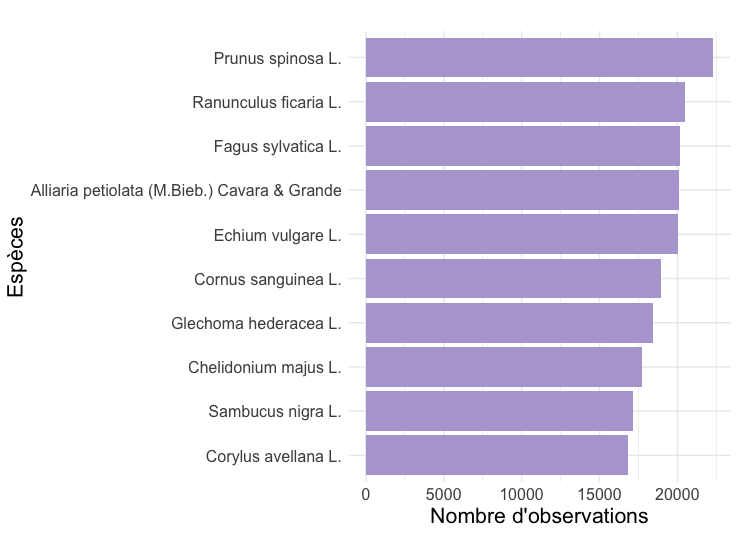
\includegraphics[scale=0.3]{images/10_Most_Observed_Species.png}
  \label{fig1}
\end{figure}

Nous pouvons lire ci-dessus les appellations des dix espèces les plus photographiées. Ce sont essentiellement des arbres vivaces, certains fruitiers, ou des fleurs comestibles, aux propriétés curatives qui peuvent être aperçues dans toute la zone géographique qui nous intéresse. 

\vspace{0.2cm}

Le \textit{Prunus Spinosa L.} ou, plus communément, prunellier est l'espèce qui revient le plus souvent, nous la verrons apparaître dans la majorité des graphes qui vont suivre. Parmi les espèces les moins observées, nous n'avons pas retenu de particularités qui les relieraient mais il est très probable que ce soient des plantes plus rares ou qui suscitent moins l'intérêt de l'observateur.

\vspace{0.2cm}

Au-delà de la répartition des apparitions des espèces qui semble seulement impliquer un intérêt de l'observateur, nous nous sommes intéressées aux scores top $1$ apportés par l'IA de Pl@ntNet, c'est-à-dire à l'espèce prédite ayant la plus grande probabilité d'être correcte pour une photographie donnée. Nous avons donc obtenu les graphiques suivants :

\begin{figure}[H]
\centering
\begin{minipage}{0.5\textwidth}
  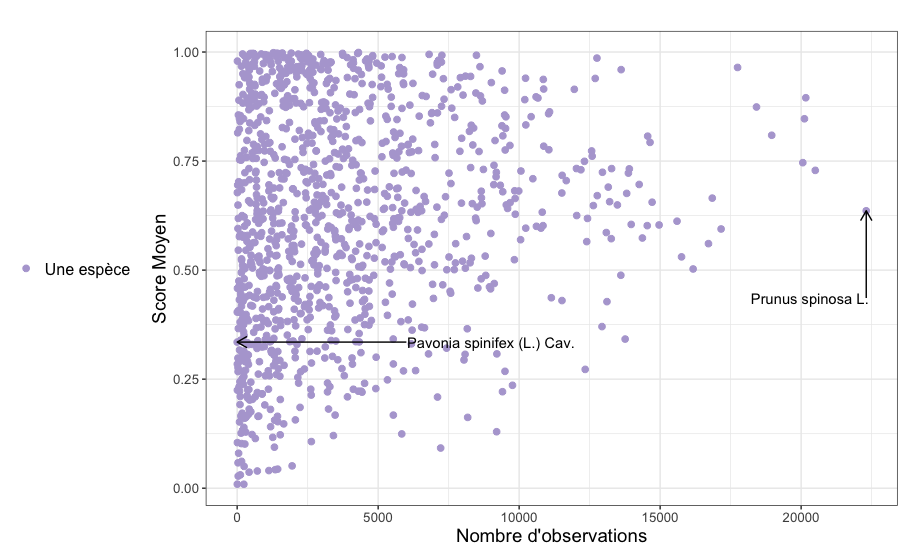
\includegraphics[width=0.8\linewidth]{images/mean_rd.png}
\end{minipage}%
\begin{minipage}{0.5\textwidth}
  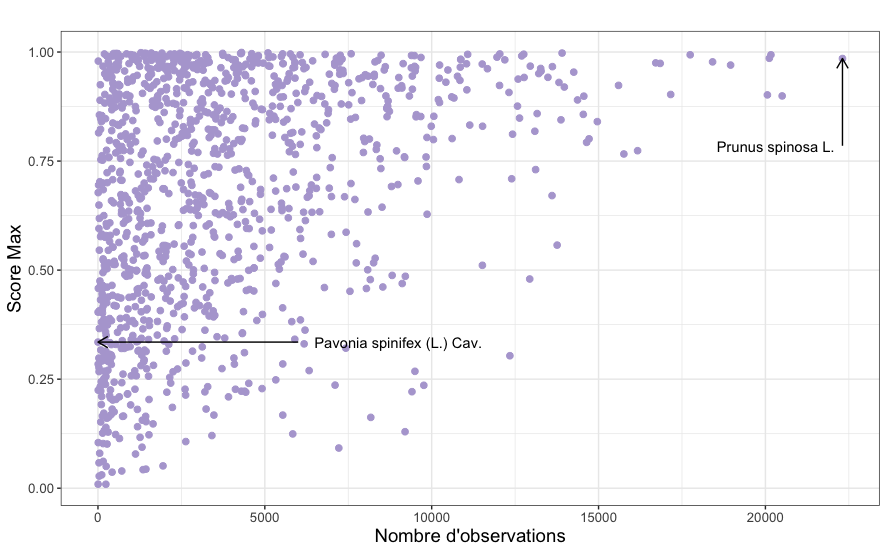
\includegraphics[width=0.8\linewidth]{images/max_rd.png}
\end{minipage}
\end{figure}

Le premier graphe représente la moyenne des probabilités de toutes les observations pour une même espèce par rapport au nombre d'occurrences de cette dernière. Quant au second graphe, il représente le maximum de ces probabilités. Chaque point violet représente une photographie prise par un observation.
Nous avons mis en relief une espèce n'ayant été observée qu'une seule fois dans ce jeu de données, \textit{Pavonia spinifex (L.) Cav.} et le prunellier déjà cité.

\vspace{2.0cm}

À première vue, il n'y a pas de relation évidente entre la fréquence d'apparitions et les scores de l'IA. Nous remarquons tout de même que le prunellier a en moyenne un score Top 1 assez proche de 1 et que le pavonia spinifex a un score assez bas, et la répartition des points sur les deux graphes est similaire, ce sont les mêmes 2000 espèces aléatoirement désignées qui sont présentées.

\vspace{2.0cm}

Nous avons quelques hypothèses permettant de comprendre pourquoi certaines espèces vues une seule fois peuvent avoir de très bon scores et pourquoi, au contraire, certaines espèces fréquentes peuvent avoir des scores presque nuls. Tout d'abord, la qualité de l'image : si l'objectif est trop éloigné, si l'image est floue, s'il y a des objets qui font obstacle (un emballage plastique transparent par exemple) ou s'il y a plusieurs espèces dans la même image, alors la performance de l'IA en est lésée.
Ensuite, il se peut que l'IA ait été entraînée sur des images d'une espèce qui, dans notre base de données, n'apparaît qu'une seule fois. Ainsi, pour l'IA, c'est une espèce qu'elle sait reconnaître à chaque fois car elle existe dans sa base d'entraînement comme la même photographie. Ainsi, la plante peut se voir octroyer un score élevé même dans notre jeu de données.

...

%%%%%%%%%%%%%%%%%%%%%%%%%%%%%%%%%%%%%%%%%%%%%%%%%%%%%%%%%%%%%%%%%%%%%%%%%%%%%%%%

\subsection{Prédiction conforme}

La prédiction conforme permet de quantifier l'incertitude des prédictions faites par des algorithmes de prédiction arbitraire (ref). C'est-à-dire convertir les prédictions d'un algorithme en un ensemble de prédictions qui ont de fortes probabilités de contenir la réponse correcte.
% * <aigoin.emilie@gmail.com> 12:02:29 29 Mar 2025 UTC+0100:
% mettre ref

\vspace{0.2cm}

Nous avons $(X_i, Y_i)$ des paires constituées de caractéristiques ($X_i$) et de réponses ($Y_i$) indépendants et identiquement distribués issus d'une distribution $P$, avec $i = 1, \dots, n$. Notre espace des caractéristiques est $X = \mathbb R^d$ et notre espace des réponses est $Y = \mathbb R$.

\vspace{0.2cm}

Nous fixons un niveau d'erreur $\alpha \in ]0,1[$.

\vspace{0.2cm}

Ainsi, nous cherchons à construire un intervalle $\hat C_n (X_{n+1})$ qui contienne $Y_{n+1}$ avec une probabilité d'au moins $1- \alpha$, c'est-à-dire : $$ \mathbb P(Y_{n+1} \in \hat C_n (X_{n+1}) \geq 1 - \alpha) $$

\vspace{0.2cm}

Tout cela nécessite certaines conditions. La première va être de ne pas poser d'hypothèse sur $P$. Nous ne devons pas non plus utiliser toutes les prédictions possibles car nous voulons un nombre de précision fini mais également raisonnable. Pour finir, nous voulons adapter notre stratégie à la dureté du problème, c'est-à-dire que plus il est facile de prédire $Y_{n+1}$ à partir de $X_{n+1}$ et plus notre ensemble $\hat C_n(X_{n+1})$ devra être petit.

\vspace{0.2cm}

Cela est tout à fait possible avec une distribution infinie dans des conditions standard (convergence du quantile de l'échantillon vers le quantile de la population). Mais, étant donné que nous sommes dans des conditions réelles, nous nous intéressons ici à des échantillons finis.

%%%%%%%%%%%%%%%%%%%%%%%%%%%%%%%%%%%%%%%%%%%%%%%%%%%%%%%%%%%%%%%%%%%%%%%%%%%%%%%%

\subsection{Algorithmes de prédiction}

Le premier algorithme que nous avons utilisé est celui de la prédiction conforme de Vovk et al.  qui permet d'obtenir le score de la bonne classe.
% * <aigoin.emilie@gmail.com> 12:33:22 29 Mar 2025 UTC+0100:
% ajouter ref

\vspace{0.2cm}

Le deuxième algorithme dont nous nous sommes servis est celui de Romano et al. qui nous permet d'obtenir un ensemble de prédictions adaptatifs. 
% * <aigoin.emilie@gmail.com> 12:34:34 29 Mar 2025 UTC+0100:
% ajouter ref 

Pour cela, il faut tout d'abord commencer par ordonner les classes en fonction de leurs scores dans l'ordre décroissant. Puis, prendre la somme des sorties softmax jusqu'à atteindre la vraie classe (formule) (graphique).
% * <aigoin.emilie@gmail.com> 12:36:32 29 Mar 2025 UTC+0100:
% ajouter formule et graphique


%%%%%%%%%%%%%%%%%%%%%%%%%%%%%%%%%%%%%%%%%%%%%%%%%%%%%%%%%%%%%%%%%%%%%%%%%%%%%%%%
%%%%%%%%%%%%%%%%%%%%%%%%%%%%%%%%%%%%%%%%%%%%%%%%%%%%%%%%%%%%%%%%%%%%%%%%%%%%%%%%

\section{Conclusion}



\printbibliography

\end{document}

